\documentclass[submit]{harvardml}

% Put in your full name and email address.
\name{Luke Mueller}
\email{lam908@mail.harvard.edu}

% List any people you worked with.
\collaborators{%
  Nicole Lee,
  Dong Yan
}

% You don't need to change these.
\course{CS181-S16}
\assignment{Assignment \#1}
\duedate{5:00pm February 5, 2016}

\usepackage[OT1]{fontenc}
\usepackage[colorlinks,citecolor=blue,urlcolor=blue]{hyperref}
\usepackage[pdftex]{graphicx}
\usepackage{subfig}
\usepackage{fullpage}
\usepackage{palatino}
\usepackage{mathpazo}
\usepackage{amsmath}
\usepackage{amssymb}
\usepackage{color}
\usepackage{todonotes}
\usepackage{listings}
\usepackage{common}

\usepackage[mmddyyyy,hhmmss]{datetime}

\definecolor{verbgray}{gray}{0.9}

\lstnewenvironment{csv}{%
  \lstset{backgroundcolor=\color{verbgray},
  frame=single,
  framerule=0pt,
  basicstyle=\ttfamily,
  columns=fullflexible}}{}


\begin{document}
\begin{center}
{\Large Homework 1: Linear Regression}\\
\end{center}
You should submit your answers as a PDF via the Canvas course website.  There is a mathematical component and a programming component to this homework.You may collaborate with others, but are expected to list collaborators, and write up your problem sets individually.\\

\noindent
Please type your solutions after the corresponding problems using this \LaTeX\ template, and start each problem on a new page.\\

%%%%%%%%%%%%%%%%%%%%%%%%%%%%%%%%%%%%%%%%%%%%%
% Problem 1
%%%%%%%%%%%%%%%%%%%%%%%%%%%%%%%%%%%%%%%%%%%%%
\begin{problem}[Centering and Ridge Regression, 7pts]
%\subsection*{1. Centering and Ridge Regression [7pts]}

Consider a data set in which each data input vector $\boldx \in \mathbb{R}^m$. Let $\boldX \in
\mathbb{R}^{n \times m}$ be the input matrix, the rows of which are the input
vectors, and the columns of which are centered at 0. Let $\lambda$ be a positive constant. We define:

$$J(\boldw, w_0) = (\boldy - \boldX \boldw - w_0 {\bf 1 })^T (\boldy - \boldX
\boldw - w_0 {\bf 1 }) + \lambda \boldw^T \boldw$$

\begin{itemize}
  \item[(a)] Compute the gradient of $J(\boldw, w_0)$ with respect to $w_0$.
    Simplify as much as you can for full credit.
  \item[(b)] Compute the gradient of $J(\boldw, w_0)$ with respect to $\boldw$.
    Simplify as much as you can for full credit. Make sure to give your answer
    in matrix form.
  \item[(c)] Suppose that $\lambda > 0$. Knowing that $J$ is a convex function
    of its arguments, conclude that a global optimizer of
    $J(\boldw, w_0)$ is
    \begin{align}
      w_0 &= \frac{1}{n} \sum_i y_i \\
      \boldw &= (\boldX^T \boldX + \lambda \boldI)^{-1} \boldX^T \boldy
    \end{align}
    Before taking the inverse of a matrix, prove that it is invertible.
\end{itemize}
\end{problem}

\subsubsection*{Solution}

$J(\boldw, w_0) = (\boldy - \boldX \boldw - w_0 {\bf 1 })^T (\boldy - \boldX
\boldw - w_0 {\bf 1 }) + \lambda \boldw^T \boldw$ \\

$ = \boldy^T\boldy - \boldy\boldX\boldw - \boldy^T w_0 \bf 1 - (\boldX\boldw)^T\boldy + (\boldX\boldw)^T(\boldX\boldw) + (\boldX\boldw)^T w_0 \bf 1 - w_0 \bf 1 \boldy^T + w_0 \bf 1^T(\boldX\boldw) + w_0^2 \bf 1^T {\bf 1} + \lambda \boldw^T \boldw$ \\

\noindent
$\nabla J_{w_0} = -\boldy^T\bf 1 + (\boldX\boldw)^T\bf 1 - \bf 1^T\boldy + \bf 1^T(\boldX\boldw) + 2w_0 \bf 1^T\bf 1 $ \\

\noindent
Then, $\boldX^T\bf 1 = \bf 1^T\boldX = 0$ since we are taking the sum of columns, which are centered at $0$. This also implies $(\boldX\boldw)^T \bf 1 = \boldw^T\boldX^T\bf 1= 0$. In addition, $-\boldy^T\bf 1 = - \bf 1^T\boldy = -\sum_i y_i$, and $\bf 1^T \bf 1 = n$ thus we have:

$$ \nabla J_{w_0} = -2\sum_i y_i + 2w_0n$$

\pagebreak
\noindent
For part (b), first we extract terms relevant to $\nabla J_{\boldw}$: 
\\\\
$-\boldy^T\boldX\boldw - (\boldX\boldw)^T\boldy + (\boldX\boldw)^T(\boldX\boldw) + (\boldX\boldw)^T w_0 \bf 1 + w_0 \bf 1^T (\boldX\boldw) + \lambda\boldw^T\boldw $
\\\\
Then as before, and since $w_0$ is a scalar, we have $(\boldX\boldw)^T w_0 \bf 1 = w_0 \bf 1^T (\boldX\boldw) = 0$. Taking the remaining partial derivatives and combining terms the gradient is thus:

$$ \nabla J_{\boldw} = -2\boldy^T\boldX + 2\boldw^T\boldX^T\boldX + 2\lambda\boldw^T$$
\\
\noindent 
For part (c) we first return to the gradient of $\nabla J_{w_0}$. Since we have the partial derivative of $J$ with respect to $w_0$, we can determine the global optimizer of $J(\boldw, w_0)$ by setting the gradient equal to $0$. Thus we have:

$$-2\sum_i y_i + 2w_0n = 0 \Rightarrow -2\sum_i y_i = 2w_0n \Rightarrow \sum_i y_i = w_0n \Rightarrow w_0 = \frac{1}{n}\sum_i y_i $$
\\
\noindent
Solving for $\boldw$ is a similar process, though slightly less trivial. First, we prove $\boldX^T\boldX+\lambda\boldI$ is invertible for a later purpose, using the following property: if $det(A) \neq 0$, then $A$ is invertible.

$$det(\boldX^T\boldX+\lambda\boldI) = det(\boldX^T\boldX)+det(\lambda\boldI) = det(\boldX^T)det(\boldX)+det(\lambda\boldI)$$

\noindent
Then, since we previously showed that $\boldX^T\bf 1 = 0$ it follows that there exists a nontrivial solution to $det(\boldX)$, thus $det(\boldX)=0$. Therefore:
$$det(\boldX^T\boldX+\lambda\boldI) = 0 + det(\lambda\boldI) = \lambda\neq 0 $$ $\Rightarrow \boldX^T\boldX+\lambda\boldI$ is invertible.
\\\\
\noindent
Now returning to $ \nabla J_{\boldw}$, we set the gradient equal to $0$ to determine the global optimizer. $$\nabla J_{\boldw}= -2\boldy^T\boldX + 2\boldw^T\boldX^T\boldX + 2\lambda\boldw^T = 0$$
$$ -\boldy^T\boldX + \boldw^T\boldX^T\boldX + \lambda\boldw^T = 0 $$
$$ \boldy^T\boldX = \boldw^T\boldX^T\boldX + \lambda\boldw^T $$
$$ \boldX^T\boldy = \boldX^T\boldX\boldw + \lambda\boldw $$
$$ \boldX^T\boldy = (\boldX^T\boldX + \lambda\bf I)\boldw $$
$$ (\boldX^T\boldX + \lambda\bf I)^{-1} \boldX^T\boldy = \boldw $$



%%%%%%%%%%%%%%%%%%%%%%%%%%%%%%%%%%%%%%%%%%%%%
% Problem 2
%%%%%%%%%%%%%%%%%%%%%%%%%%%%%%%%%%%%%%%%%%%%%
\newpage
%\subsection*{2. Priors and Regularization [7pts]}
\begin{problem}[Priors and Regularization,7pts]
Consider the Bayesian linear regression model given in Bishop 3.3.1. The prior is
\begin{align*}
p(\boldw \given \alpha) = \mathcal{N}(\boldw \given \bold0, \alpha^{-1}\ident ),
\end{align*}
where $\alpha$ is the precision parameter that controls the variance of the Gaussian prior.  The likelihood can be written as
\begin{align*}
p(\boldt \given \boldw) &= \prod_{n=1}^N \mcN(t_n \given \boldw^\trans \bphi(\boldx_n), \beta^{-1}),
\end{align*}

Using the fact that the posterior is the product of the prior and the likelihood (up to a normalization constant), show that maximizing the log posterior (i.e., $\ln p(\boldw \given \boldt)= \ln p(\boldw | \alpha) + \ln p(\boldt \given \boldw)$) is equivalent to minimizing the regularized error term given by ${E_D(\boldw) + \lambda E_W(\boldw)}$ with 
\begin{align*}
E_D(\boldw) &= \frac{1}{2}\sum_{n = 1}^N (t_n - \boldw^\trans \bphi(\boldx_n))^2 \\
E_W(\boldw) &= \frac{1}{2}\boldw^\trans \boldw
\end{align*} 

Do this by writing $\ln p(\boldw \given \boldt)$ as a function of $E_D(\boldw)$ and $E_W(\boldw)$, dropping constant terms if necessary.  Conclude that maximizing this posterior is equivalent to minimizing the regularized error term given by $E_D(\boldw) + \lambda E_W(\boldw)$. (Hint: take $\lambda = \alpha/\beta$)
\end{problem}


\subsubsection*{Solution}
Starting with the prior:

$$p(\boldw \given \alpha) = \mathcal{N}(\boldw \given \bold0, \alpha^{-1}\ident ) = \frac{1}{{\sqrt {2\pi\alpha^{-1}\ident} }}e^{{{ - \left( {\boldw - \bf 0 } \right)^2 } \mathord{\left/ {\vphantom {{ - \left( {\boldw - \bf 0 } \right)^2 } {2\alpha^{-1}\ident }}} \right. \kern-\nulldelimiterspace} {2\alpha^{-1}\ident }}}$$

\noindent
Taking the natural log and removing irrelevant terms (i.e. constants, since the posterior need only be proportional) we are left with:

$$\frac{(\boldw - \bf 0)^2}{2\alpha^{-1}\ident} = \frac{1}{2\alpha^{-1}\ident}\boldw^\trans \boldw = \frac{E_W(\boldw)}{\alpha^{-1}\ident}$$

\noindent
Now for the likelihood:
$$ p(\boldt \given \boldw) = \prod_{n=1}^N \mcN(t_n \given \boldw^\trans \bphi(\boldx_n), \beta^{-1}) = \frac{1}{{\sqrt {2\pi\beta^{-1}} }}e^{{{ - \left( {t_n - \boldw^\trans \bphi(\boldx_n) } \right)^2 } \mathord{\left/ {\vphantom {{ - \left( {t_n - \boldw^\trans \bphi(\boldx_n) } \right)^2 } {2\beta^{-1} }}} \right. \kern-\nulldelimiterspace} {2\beta^{-1} }}} $$

\noindent
As before, taking the natural log and removing irrelevant terms we are left with:
$$ \frac{1}{2\beta^{-1}}\sum_{n = 1}^N (t_n - \boldw^\trans \bphi(\boldx_n))^2 = \frac{E_D(\boldw)}{\beta^{-1}} $$

\noindent
Now combining the prior and likelihood through the sum of natural logs we have:
$$ \ln p(\boldw \given \boldt) = \frac{E_D(\boldw)}{\beta^{-1}} + \frac{E_W(\boldw)}{\alpha^{-1}\ident}$$

\noindent
Then multiplying by $\beta^{-1}$ and defining $\lambda = \alpha/\beta$ we have:
$$ \ln p(\boldw \given \boldt) = E_D(\boldw) + \lambda E_W(\boldw) $$


%%%%%%%%%%%%%%%%%%%%%%%%%%%%%%%%%%%%%%%%%%%%%
% Problem 3
%%%%%%%%%%%%%%%%%%%%%%%%%%%%%%%%%%%%%%%%%%%%%
\newpage
\subsection*{3. Modeling Changes in Congress [10pts]}
 The objective of this problem is to learn about linear regression with basis
 functions by modeling the average age of the US Congress. The file
 \verb|congress-ages.csv| contains the data you will use for this problem.  It
 has two columns.  The first one is an integer that indicates the Congress
 number. Currently, the 114th Congress is in session. The second is the average
 age of that members of that Congress.  The data file looks like this:
\begin{csv}
congress,average_age
80,52.4959
81,52.6415
82,53.2328
83,53.1657
84,53.4142
85,54.1689
86,53.1581
87,53.5886
\end{csv}
and you can see a plot of the data in Figure~\ref{fig:congress}.

\begin{figure}[h]
\centering
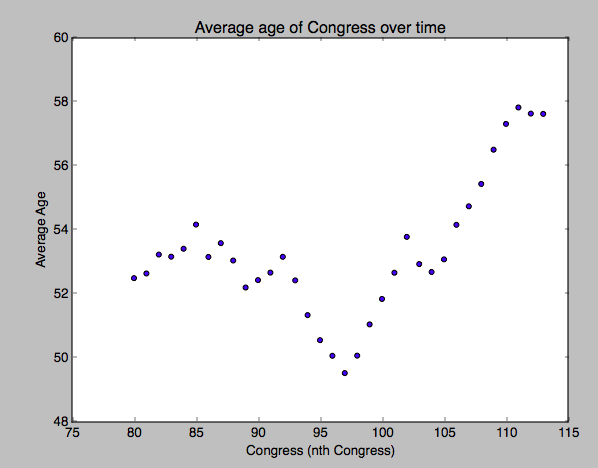
\includegraphics[width=0.8\textwidth]{congress-ages}
\caption{Average age of Congress.  The horizontal axis is the Congress number, and the vertical axis is the average age of the congressmen.}
\label{fig:congress}
\end{figure}

\begin{problem}[Modeling Changes in Congress, 10pts]
Implement basis function regression with ordinary least squares with the above
data. Some sample Python code is provided in \verb|linreg.py|, which implements
linear regression.  Plot the data and regression lines for the simple linear
case, and for each of the following sets of basis functions:
\begin{itemize}
	\item[(a)] $\phi_j(x) = x^j$ for $j=1, \ldots, 7$
	\item[(b)] $\phi_j(x) = x^j$ for $j=1, \ldots, 3$
	\item[(c)] $\phi_j(x) = \sin\{ x / j \}$ for $j=1, \ldots, 4$
	\item[(d)] $\phi_j(x) = \sin\{ x / j \}$ for $j=1, \ldots, 7$
	\item[(e)] $\phi_j(x) = \sin\{ x / j \}$ for $j=1, \ldots, 20$
\end{itemize}
  In addition to the plots, provide one or two sentences for each, explaining
  whether you think it is fitting well, overfitting or underfitting.  If it does
  not fit well, provide a sentence explaining why. A good fit should capture the
  most important trends in the data.
	\end{problem}

\subsubsection*{Solution}

\begin{figure}[h]
\centering
\includegraphics[width=0.8\textwidth]{graph_a}
\caption{Graph for part A. The fit appears to do well in this plot, except in the lower tail where the data do not reflect the trend line. However, the main concern here is overfitting. We have only 34 data points, yet we are using 7 coefficients to perform our regression.}
\label{fig:grapha}
\end{figure}

\begin{figure}[h]
\centering
\includegraphics[width=0.8\textwidth]{graph_b}
\caption{Graph for part B. The fit is not as good as in part (a), and we definitely don't seem to be capturing any useful information in the tails (which seem to plateau somewhat). But here we use far fewer degrees of freedom (coefficients) to fit the regression, which is a plus.}
\label{fig:graphb}
\end{figure}

\begin{figure}[h]
\centering
\includegraphics[width=0.8\textwidth]{graph_c}
\caption{Graph for part E. This plot is more or less a compromise of the previous plots, since it uses fewer degrees of freedom than (a) yet provides slightly better fit than (b). However, it seems like we could get by with fewer degrees of freedom since there are some unnecessary "wiggles" in the regression line. Also, there is a disconnect between the data and the regression line in the tails.}
\label{fig:graphc}
\end{figure}

\begin{figure}[h]
\centering
\includegraphics[width=0.8\textwidth]{graph_d}
\caption{Graph for part D. This plot is more accurate than plot (c), capturing the information in the tails far better than before. However, as in part (a) we are using many degrees of freedom so there is concern for overfitting.}
\label{fig:graphd}
\end{figure}

\begin{figure}[h]
\centering
\includegraphics[width=0.8\textwidth]{graph_e}
\caption{Graph for part E. Obviously, this is the best fit of any plot so far. With so many degrees of freedom, we capture nearly every point perfectly. However, the overfitting is too much to make any meaningful inference. Perhaps the only use here is identifying potential outliers (i.e., between 100-105th congress).}
\label{fig:graphe}
\end{figure}

%%%%%%%%%%%%%%%%%%%%%%%%%%%%%%%%%%%%%%%%%%%%%
% Problem 4
%%%%%%%%%%%%%%%%%%%%%%%%%%%%%%%%%%%%%%%%%%%%%
\clearpage
\begin{problem}[Calibration, 1pt]
Approximately how long did this homework take you to complete?
\end{problem}
\textbf{Answer:}
\\
\noindent
7 hours. 2-3 hours LaTeX (beginner), 1-2 hours python, 3-4 (or more) working out problem 1 and 2. My linear algebra is very rusty!






\end{document}
